\section{Results and Analysis}\label{sec:4}
\graphicspath{ {../} }
    The results of each image are show in order of size. Note: each value is the integer median of 10 repetitions and the wait() was commented.\\

    Image sample appearance:

    \begin{figure}[h!]
        \caption{Sample - Image 1}
        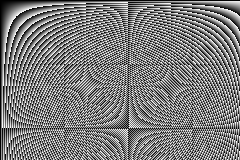
\includegraphics{sample.png}
    \end{figure}

\begin{table}[h!]
    \centering
    \caption{Milliseconds Performance}
    \label{tab1}
        \begin{tabular}{ccccccc}
        \hline
            & \multicolumn{2}{c}{1280x720} & \multicolumn{2}{c}{4320x1280} & \multicolumn{2}{c}{8640x4320} \\\hline
        cv1 & 98ms          & 05ms         & 133ms         & 129ms         & 418ms         & 271ms         \\\hline
        cv2 & 104ms         & 06ms         & 141ms         & 38ms          & 365ms         & 255ms         \\\hline
            & all           & loop         & all           & loop          & all           & loop          \\\hline
\end{tabular}
\end{table}

    The results shows that the simplicity of code image 1280x720 can be really dominated by both algorithm.  

    In the image 4320x1280 is the best view for all performance gain. It's a lot faster, mainly when just loop iteration is observed.

    In the third image, 8640x4320, the Mat() method is still faster, but suggest a convergence with iplImage(); 

    OpenCV Documentation has it's own comparative between algorithm with Mat(). And the results are corroborated. OpenCV developers call these loop-access implementation of ``Efficient Way''.  